\documentclass[a4paper, 12pt]{article}
\usepackage{lmodern}
\usepackage{url}
\usepackage{enumitem}
\usepackage{tabularx}
\usepackage{colortbl}
\usepackage{adjustbox}
\usepackage{ragged2e}
\usepackage[table]{xcolor}
\usepackage{graphicx}
\graphicspath{{./images/}}

\begin{document}
\begin{titlepage}
\title{Preliminary Analysis and Visualization: Titanic Dataset Analysis}
\author{
  Ali Khan, Salal\\
  \texttt{202307216 - x2023flb@stfx.ca}
  \and
  Aziz, Abdul\\
  \texttt{202209343 - x2023dir@stfx.ca}
  \and
  Javed, Muhammad\\
  \texttt{202303808 - x2023dvh@stfx.ca}
}
\date{Oct 29, 2023}
\maketitle
\end{titlepage}

\section*{Exploratory Data Analysis}

\mbox{}

The dataset contains information about passengers that were in Titanic, with several attributes. Here's a quick overview of the data:

\mbox{}

\begin{table}[h]
  \centering
  \begin{tabular}{|l|l|}
    \hline
    \rowcolor[HTML]{EFEFEF}
    \textbf{Column Name} & \textbf{Data Type} \\ \hline
    PassengerId & int64 \\ \hline
    Survived & int64 \\ \hline
    Pclass & int64 \\ \hline
    Name & object \\ \hline
    Sex & object \\ \hline
    Age & float64 \\ \hline
    SibSp & int64 \\ \hline
    Parch & int64 \\ \hline
    Ticket & object \\ \hline
    Fare & float64 \\ \hline
    Cabin & object \\ \hline
    Embarked & object \\ \hline
  \end{tabular}
\end{table}

\begin{table}[ht]
  \centering
  \begin{adjustbox}{width=1\textwidth}
  \begin{tabular}{rlrrrrrrrrrrr}
    \hline
    & \textbf{PassengerId} & \textbf{Survived} & \textbf{Pclass} & \textbf{Name} & \textbf{Sex} & \textbf{Age} & \textbf{SibSp} & \textbf{Parch} & \textbf{Ticket} & \textbf{Fare} & \textbf{Cabin} & \textbf{Embarked} \\
    \hline
    0 & 1 & 0 & 3 & Braund, Mr. Owen Harris & male & 22.0 & 1 & 0 & A/5 21171 & 7.2500 & NaN & S \\
    1 & 2 & 1 & 1 & Cumings, Mrs. John Bradley (Florence Briggs Th... & female & 38.0 & 1 & 0 & PC 17599 & 71.2833 & C85 & C \\
    2 & 3 & 1 & 3 & Heikkinen, Miss. Laina & female & 26.0 & 0 & 0 & STON/O2. 3101282 & 7.9250 & NaN & S \\
    3 & 4 & 1 & 1 & Futrelle, Mrs. Jacques Heath (Lily May Peel) & female & 35.0 & 1 & 0 & 113803 & 53.1000 & C123 & S \\
    4 & 5 & 0 & 3 & Allen, Mr. William Henry & male & 35.0 & 0 & 0 & 373450 & 8.0500 & NaN & S \\
    \hline
  \end{tabular}
  \end{adjustbox}
  \caption{Snapshot of `dataset.head()` displaying first 5 rows } 
\end{table}  
  
\begin{table}[ht]
  \centering
  \begin{adjustbox}{width=1\textwidth}
  \begin{tabular}{rlrrrrrrrrrrr}
    \hline
    & \textbf{PassengerId} & \textbf{Survived} & \textbf{Pclass} & \textbf{Name} & \textbf{Sex} & \textbf{Age} & \textbf{SibSp} & \textbf{Parch} & \textbf{Ticket} & \textbf{Fare} & \textbf{Cabin} & \textbf{Embarked} \\
    \hline
    886 & 887 & 0 & 2 & Montvila, Rev. Juozas & male & 27.0 & 0 & 0 & 211536 & 13.00 & NaN & S \\
    887 & 888 & 1 & 1 & Graham, Miss. Margaret Edith & female & 19.0 & 0 & 0 & 112053 & 30.00 & B42 & S \\
    888 & 889 & 0 & 3 & Johnston, Miss. Catherine Helen "Carrie" & female & NaN & 1 & 2 & W./C. 6607 & 23.45 & NaN & S \\
    889 & 890 & 1 & 1 & Behr, Mr. Karl Howell & male & 26.0 & 0 & 0 & 111369 & 30.00 & C148 & C \\
    890 & 891 & 0 & 3 & Dooley, Mr. Patrick & male & 32.0 & 0 & 0 & 370376 & 7.75 & NaN & Q \\
    \hline
  \end{tabular}
  \end{adjustbox}
  \caption{Snapshot of `dataset.tail()` displaying last 5 rows } 
\end{table} 

\begin{table}[h]
  \centering
  \begin{tabular}{lr}
    \hline
    \textbf{Column Name} & \textbf{Count} \\
    \hline
    Survived & 2 \\
    Pclass & 3 \\
    Name & 891 \\
    Sex & 2 \\
    Age & 88 \\
    SibSp & 7 \\
    Parch & 7 \\
    Ticket & 681 \\
    Fare & 248 \\
    Cabin & 147 \\
    Embarked & 3 \\
    \hline
  \end{tabular}
  \caption{Sum of unique values for each column}
  \paragraph*{}
  \justifying
Analyzing the number of unique values in each attribute of dataset is essential for data quality assessment, identifying data patterns, and guiding data preprocessing and modeling decisions in data analysis. 
\end{table} 

\begin{table}[h]
  \centering
  \begin{tabular}{lr}
    \hline
    \textbf{Column Name} & \textbf{Count} \\
    \hline
    Survived & 0 \\
    Pclass & 0 \\
    Name & 0 \\
    Sex & 0 \\
    Age & 177 \\
    SibSp & 0 \\
    Parch & 0 \\
    Ticket & 0 \\
    Fare & 0 \\
    Cabin & 687 \\
    Embarked & 2 \\
    \hline
  \end{tabular}
  \caption{Sum of null values for each column} 
  \paragraph*{}
  \justifying
Checking for missing values (null values) plays an important role in data analysis because it helps us to spot problems in dataset and we train the data on meaningful and complete data. After checking the null values We need to decide what to do with missing data, like filling in the gaps if they are less in number or removing them if the null count is very large and column is not meaningful for training the model, to avoid errors and unfair results.
\end{table} 

\begin{table}[h]
  \centering
  \begin{tabular}{lr}
    \hline
    \textbf{Column Name} & \textbf{Mean} \\
    \hline
    Age & 29.699118 \\
    Fare & 32.204208 \\
    SibSp & 0.523008 \\
    Parch & 0.381594 \\
    \hline
  \end{tabular}
  \caption{Mean of the meaningful attributes} 
  \paragraph*{Mean}
  \justifying
Calculating the mean for attributes like "Age", "Fare", "Number of Siblings", or "Number of Parents" gives us the average of columns that we need, helping to understand the average passenger's age, ticket price, number of parents or siblings accompanying passenger. It's useful for pricing analysis and finding the central value in numerical data.
\end{table} 

\begin{table}[h]
  \centering
  \begin{tabular}{lr}
    \hline
    \textbf{Column Name} & \textbf{Median} \\
    \hline
    Age & 28.0 \\
    Fare & 14.4542 \\
    \hline
  \end{tabular}
  \caption{Median of the meaningful attributes} 
  \paragraph*{Median}
  \justifying
Calculating the median of "Fare" and "Age", especially for attributes like "Age," helps us find the middle value or inter-quartile range, which is less affected by extreme ages. This is important to understand the age distribution and ensure that extreme ages don't overly influence our analysis, likewise for fare the fares might be skewed by some high class passengers while most of the passengers might paid very low fare.
\end{table} 

\begin{table}[h]
  \centering
  \begin{tabular}{lr}
    \hline
    \textbf{Column Name} & \textbf{Mode} \\
    \hline
    Survived & 0 \\
    Sex & male \\
    Pclass & 3 \\
    Embarked & S \\
    \hline
  \end{tabular}
  \caption{Mode of the meaningful attributes} 
  \paragraph*{Mode}
  \justifying
Calculating the mode for attributes in the dataset, like the most common gender, passenger class, survival status, and most common embarkation, helps us figure out what most people were like on the Titanic and make decisions about services. It also shows if there are any problems with the data and who or what is most common.
\end{table} 

\begin{table}[h]
  \centering
  \begin{tabular}{lr}
    \hline
    \textbf{Column Name} & \textbf{Range} \\
    \hline
    PassengerId & 1 - 891 \\
    Survived & 0 - 1 \\
    Pclass & 1 - 3 \\
    Age & 0.42 - 80.0 \\
    SibSp & 0 - 8 \\
    Parch & 0 - 6 \\
    Fare & 0.0 - 512.3292 \\
    \hline
  \end{tabular}
  \caption{Range of the attributes} 
  \paragraph*{Range}
  \justifying
Calculating the range of numeric attributes provides insight into the distribution of data variables within the dataset.
\end{table} 

\begin{table}[h]
\section*{Statistical Measures}
  \centering
  \begin{tabular}{|r|r|r|r|r|r|r|r|}
    \hline
    \textbf{Percentile} & \textbf{Pclass} & \textbf{Age} & \textbf{Fare} \\
    \hline
    0.25 & 2.0 & 20.125 & 7.9104 \\
    0.50 & 3.0 & 28.000 & 14.4542 \\
    0.75 & 3.0 & 38.000 & 31.0000 \\
    \hline
  \end{tabular}
  \caption{Quantile of attributes} 
  \paragraph*{Quantile}
  \justifying
Quantiles in this dataset are important for summarizing attributes like age and fare. Quantile returns the range of values of the attributes of three portions such as 25\%, 50\%, and 75\% portions. It enables decision-making, and are key for statistical analysis, allowing comparisons and pattern detection within specific data ranges.
\end{table} 

\begin{table}[h]
  \centering
  \begin{tabular}{|r|r|r|r|r|r|r|}
    \hline
    & \textbf{Survived} & \textbf{Pclass} & \textbf{Age} & \textbf{SibSp} & \textbf{Parch} & \textbf{Fare} \\
    \hline
    \textbf{Survived} & 1.000000 & -0.338481 & -0.077221 & -0.035322 & 0.081629 & 0.257307 \\
    \textbf{Pclass} & -0.338481 & 1.000000 & -0.369226 & 0.083081 & 0.018443 & -0.549500 \\
    \textbf{Age} & -0.077221 & -0.369226 & 1.000000 & -0.308247 & -0.189119 & 0.096067 \\
    \textbf{SibSp} & -0.035322 & 0.083081 & -0.308247 & 1.000000 & 0.414838 & 0.159651 \\
    \textbf{Parch} & 0.081629 & 0.018443 & -0.189119 & 0.414838 & 1.000000 & 0.216225 \\
    \textbf{Fare} & 0.257307 & -0.549500 & 0.096067 & 0.159651 & 0.216225 & 1.000000 \\
    \hline
  \end{tabular}
  \caption{Correlation between attributes} 
  \paragraph*{Correlation}
  \justifying
Correlation is used to determine the strength of relationship between different attributes. The values returned by corr() lies between the range of (-1, 1). -1 shows the perfect negative or inverse relation between two variables and vice versa. 0 value shows that there is no relation between the two variables. In our dataset correlation statistical measure telling us that Fare attribute has a strong inverse correlation with Pclass attribute meaning that the passengers who belong to higher class paid the higher fare.
\end{table} 
\clearpage
\section*{Analysis Summary}
\justifying
The analysis we have done on Titanic dataset provided us the valuable insights into the passengers demographics, including their ages, fares, genders, and rather they survived or not.
\paragraph*{}
From this analysis, we found that the majority of passengers were 31 years old and paid a fare of around 14.4542, as indicated by the median. We have also found that there are outliers that significantly influenced the fare distribution, leading to a higher mean fare of 32.204208. The analysis also shows that the gender of most of the passengers were male, embarked from location S, and traveled in class 3. Furthermore, it indicates that the majority of passengers did not survive because we have seen in the barplot that most of the females were survived.
\paragraph*{}
This analysis can help us understand the factors contributing to survival, such as the correlation between different attributes. For instance, we can now determine whether the passengers who paid the highest or lowest fares had a better chance of survival, or if traveling with siblings or parents was a crucial factor. This analysis can help us in preprocessing the data in a way that we can build a machine learning model having higher accuracy using the meaningful dataset.

\cleardoublepage

\section*{Visualization}

\subsection*{Heatmap}

\begin{figure}[h]
  \centering
  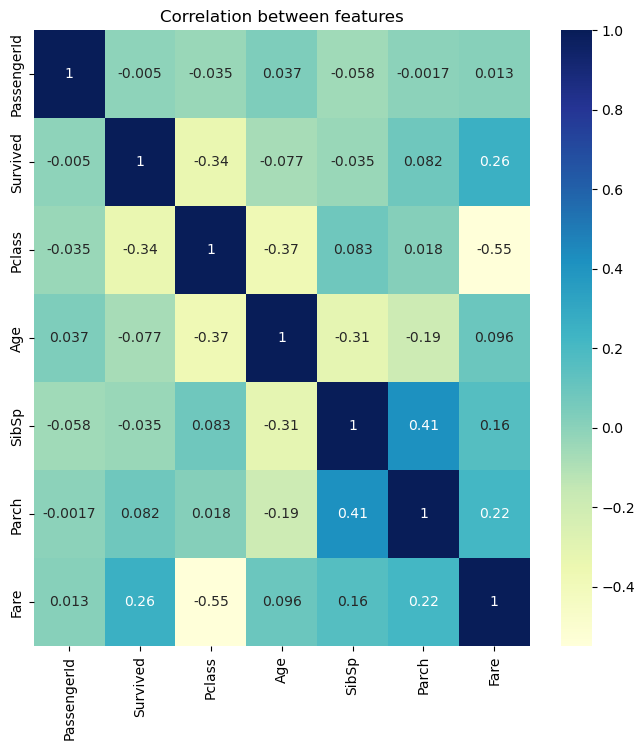
\includegraphics[width=13cm]{heatmap}
\end{figure}

Heatmap graph is showing that how much stronger the relationship of one attribute with other attributes. The greater the value of an attribute in range (-1, 1) is, the stronger the relation it shows with other attributes. Positive and negative signs are just showing the direction of relationship. In the heatmap of our dataset it is showing that SibSp and Parch columns have the strongest relationship with each other and age also have enough stronger relationship with Pclass and SibSp attribute but inversey.

\subsection*{Boxplot}

\begin{figure}[h]
  \centering
  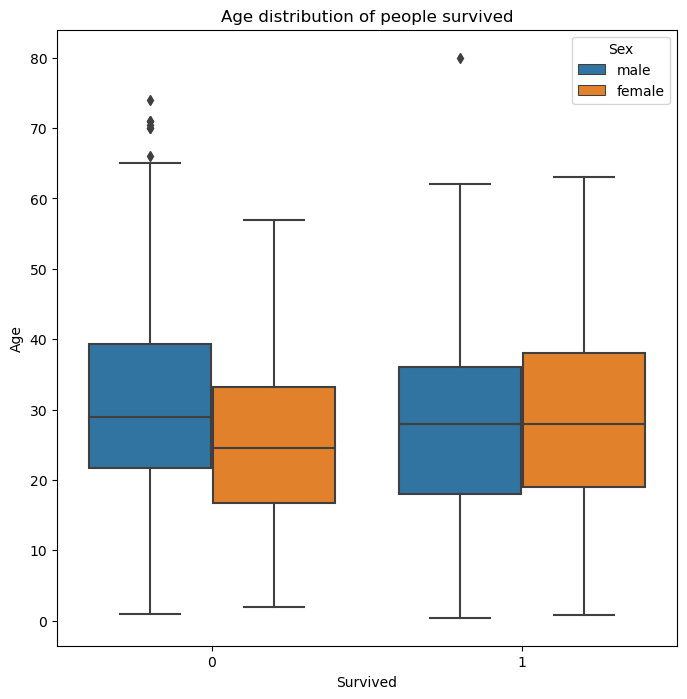
\includegraphics[width=13cm]{boxplot.png}
\end{figure}

This graph is showing the ages of males and females who were survived and not survived. This graph is also showing the outliers in the age column. The blue boxes shows the distribution of ages of males and orange boxes shows the range of ages of females. The dots are showing the outliers which is showing that there are some passengers in our dataset who were 70-80 years old.

\subsection*{Barplot}

\begin{figure}[h]
  \centering
  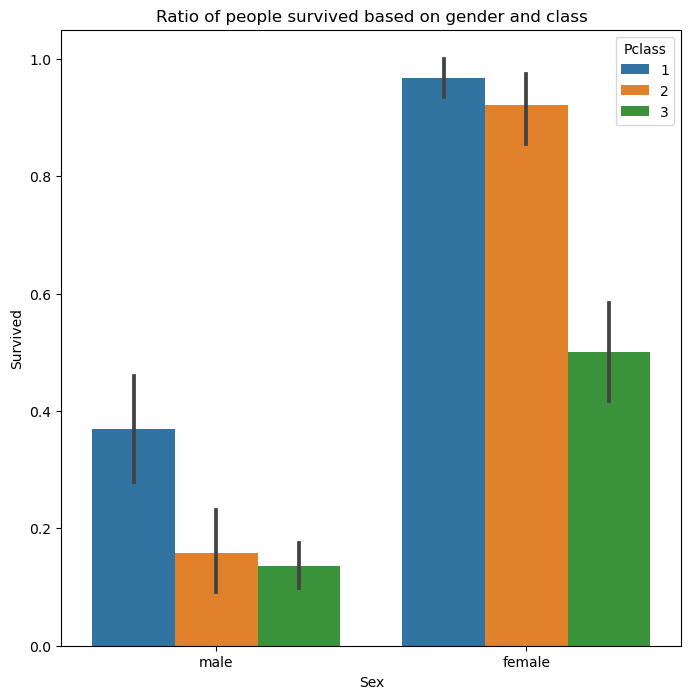
\includegraphics[width=13cm]{barplot.png}
\end{figure}

This graph shows that how many males and females survived of each class. This shows that females of each class were survived as compared to males. And most of the male and female passengers of Pclass 1 were survived.

\subsection*{Distribution Plot}

\begin{figure}[h]
    \centering
    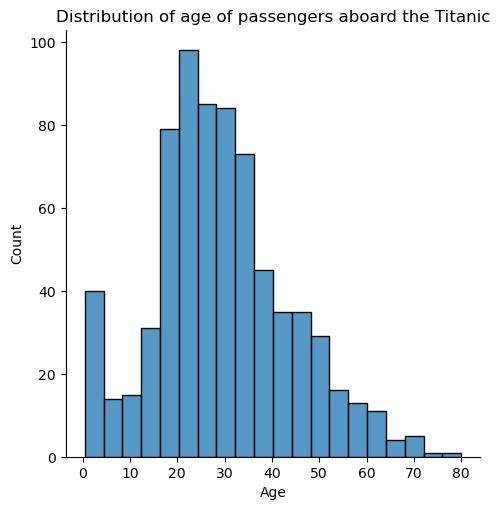
\includegraphics[width=13cm]{distplot.png}
\end{figure}

This distribution graph below shows the age distribution of the passengers who were travelling on Titanic. Higher spikes between 20 to 40 shows that most of the passengers on Titanic were 20 to 40 years old.

\subsection*{Histogram}

\begin{figure}[h]
  \centering
  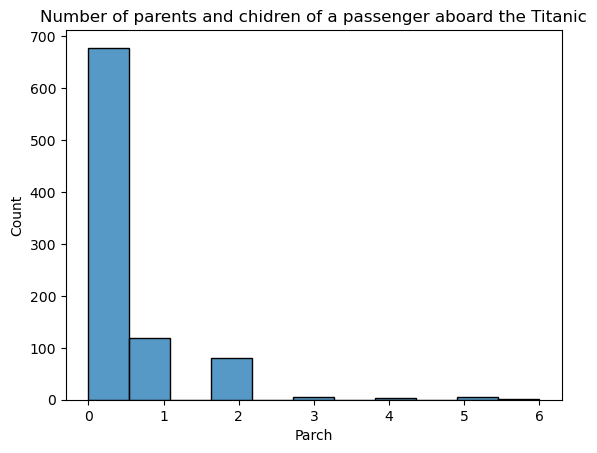
\includegraphics[width=13cm]{histplot.png}
\end{figure}

The histogram graph below shows that almost 650 passengers in our dataset didn't have any parent or children on board. Almost 110 and 90 passengers had only 1 and 2 parent or children with them respectively. Remaining passengers had more than 2 parents or children with them aboard. 

\end{document}
